\chapter{Metode}\label{chap:Metode}

%%%%%%%%%% Vision system %%%%%%%%%%
\section{Vision system}
Vision systemet i dette projekt har til formål at finde positionen af hver klods, der skal flyttes af CrustCrawleren.
Dette gøre ved brug af billeder taget med et webcam monteret ca. 1 m over det bord, CrustCrawleren er monteret på.
For at finde positionerne af klodserne oprettes en maske, der fjerner alt på billederne undtagen klodserne med en bestemt farve.
Masken oprettes ved at lede efter farver inden for fastsatte grænseværdier og fjerne farver, der ikke ligger inden for disse.
MATLAB applikationen Color Thresholder bruges til at bestemme hvilket colorspace der skal arbejdes i og hvilke grænseværdier der identificerer klodserne.
Til udvikling af vision noden i Python bruges funktioner fra OpenCV, som indeholder algoritmer relateret til computer vision.

%%%%% MATLAB - Color Thresholder %%%%%
\subsection{MATLAB - Color Thresholder}
MATLAB's  applikation Color Thresholder er blevet brugt til at bestemme, hvilket color space og hvilke grænseværdier, der er mest optimale til at identificere de farvede klodser med webcamet.

I Color Thresholder indlæses et billede, taget med webcamet, hvorpå en klods af hver farve er repræsenteret.
Valget af color space baseres på hvor klodserne adskiller sig mest fra bordpladen, da bordpladen skal fjernes med den oprettede maske.
På figur \vref{fig:ColorThresholderColorSpace} ses det, at der i color spacet HSV (Hue, Saturation, Value) er størst kontrast mellem klodser og bordplade.
Det vælges derfor at arbejde i color spacet HSV.

\figur{0.75}{ColorThresholderColorSpace.pdf}{MATLAB's applikation Color Thresholder til identifikation af optimalt color space. Den røde firkant viser, hvor der er stor kontrast mellem klodser og bordplade.}{fig:ColorThresholderColorSpace}

Color Thresholder bruges derefter til at finde grænseværdierne til hhv. H, S og V kanalerne, til identifikation af de forskelligt farvede klodser, ved at ændre på H, S og V kanalerne.
Figur \vref{fig:ColorThresholderBlue} er et eksempel på grænseværdierne til identifikation af den blå klods.

\figur{1}{ColorThresholderBlue.pdf}{Identifikation af blå klods i MATLAB's applikation Color Thresholder i color space HSV.}{fig:ColorThresholderBlue}

For hver farve blev følgende grænseværdier identificeret (se bilag \vref{app:MATLABVision} for funktioner til identifikation af hver farve):
\begin{table}[H]
\centering
\begin{tabular}{l|l|l|l}
Farve	&	H			&	S			&	V\\
\hline
Blå		&	0.515-0.790	&	0.300-1.000	&	0.400-1.000\\
Rød		&	0.900-0.080	&	0.300-1.000	&	0.000-1.000\\
Grøn	&	0.200-0.415	&	0.300-1.000	&	0.000-1.000\\
Gul		&	0.115-0.210	&	0.300-1.000	&	0.400-1.000\\
\end{tabular}	
\caption{Grænseværdier til identifikation af de fire farver, blå, rød, grøn og gul. MATLAB range 0-1.}
\end{table}

Det ses på figur \vref{fig:ColorThresholderBlue}, at nogle områder uden for bordpladen ikke forsvinder helt ved denne segmentering, da de har farver, der ligger tæt på den blå klods'.
Dette ville løses ved at beskære billedet således, at kun bordpladen vises på billedet.
Derudover skal der kun identificeres klodser på højre side af CrustCrawleren, hvorfor billedet beskæres yderligere, så kun det interessante område er vises.

Figur \vref{fig:ColorThresholderResult} viser resultatet på MATLAB analysen, som beskærer billedet og identificerer klodser i de fire farver, blå, rød, grøn og gul.
Se bilag \vref{app:MATLABVision} for script og funktioner brugt i analysen.
Det ses også på figur \ref{fig:ColorThresholderResult}, at det vil være nødvendigt at implementere en grænseværdi for hvor store områder, der skal identificeres som klodser, da der er små områder, der ikke forsvinder helt ved segmenteringen.

\figur{1}{ColorThresholderResult.pdf}{Resultat af MATLAB analysen}{fig:ColorThresholderResult}

%%%%% Vision med OpenCV-Python %%%%%
\subsection{Vision med OpenCV-Python}
Vision funktionerne, \texttt{find\_brick\_centers}, \texttt{get\_from\_webcam},\newline \texttt{extract\_single\_color\_range}, \texttt{threshold\_image}, \texttt{contours} og \texttt{get\_centers}, er udviklet i Python med det formål at identificere klodsernes placering.
Dette gøres ved at finde centrum af de klodser, der identificeres ved brug af en oprettet maske.
Den identificerer klodserne én farve af gangen og samler til sidst centrum for alle fundne klodser for alle fire farver i et array.

\texttt{find\_brick\_centers} er main funktionen til at finde centrum af klodserne, se bilag \vref{app:PythonKode} for fuld Python kode for vision funktionerne.
Funktionen starter med at definerer grænseværdierne for farverne.
OpenCV's range i HSV color spacet er ikke det samme som MATLAB's, hvorfor værdierne fundet i MATLAB skal konverteres:
\begin{table}[H]
\centering
\begin{tabular}{l|l}
H		&	0-179\\
\hline
S		&	0-255\\
\hline
V		&	0-255\\
\end{tabular}	
\caption{Range for kanalerne H, S og V i OpenCV-Python}
\end{table}

\begin{table}[H]
\centering
\begin{tabular}{l|l|l|l}
Farve	&	H			&	S			&	V	\\
\hline
Blå		&	92-141		&	76-255	&	102-255	\\
Rød		&	161-14		&	76-255	&	0-255	\\
Grøn	&	36-74		&	76-255	&	0-255	\\
Gul		&	21-38		&	76-255	&	102-255	\\
\end{tabular}	
\caption{Grænseværdier konverteret fra MATLAB range til OpenCV-Python range og afrundet til heltal.}
\end{table}

\begin{wrapfigure}{r}{0.3\textwidth}
  \begin{center}
    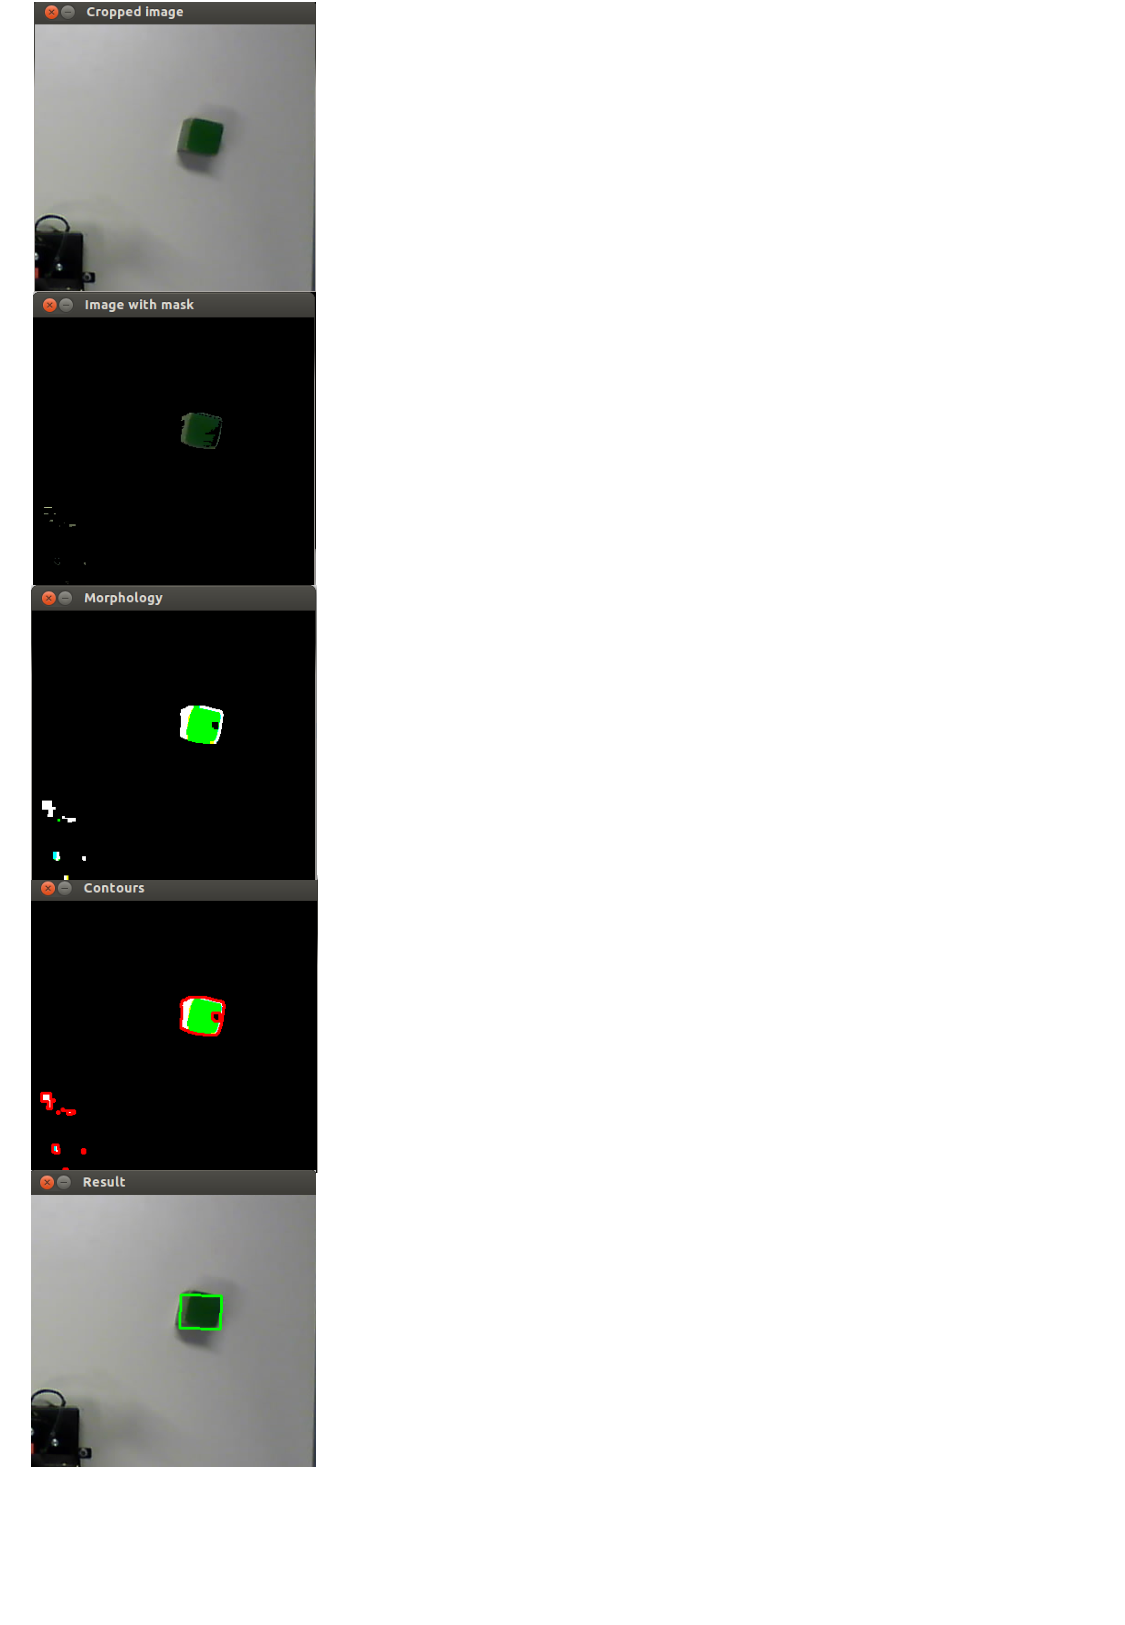
\includegraphics[width=0.23\textwidth]{figurer/ImagesFromVision}
  \end{center}
  \caption{Illustration af vision algoritmen}\label{fig:ImagesFromVision}
\end{wrapfigure}

Derudover skal H grænseværdierne for den røde klods deles op i to intervaller; 0-14 og 161-179.

Efter at have defineret grænseværdierne kaldes metoden \texttt{get\_from\_webcam}, hvilken indlæser et billede fra webcamet og beskærer det, så kun det relevante område vises på billedet.

Billedet fra \texttt{get\_from\_webcam} konverteres fra color spacet BGR til HSV ved brug af OpenCV funktionen \texttt{cv2.cvtCOLOR}.
Efter konverteringen kaldes funktionerne\newline \texttt{extract\_single\_color\_range}, \texttt{threshold\_image},\newline \texttt{contours} og \texttt{get\_centers} på billedet for hver farve.

\texttt{extract\_single\_color\_range} opretter en maske fjerner alle farver på billedet som ikke ligger i den specificerende grænseværdi, se bilag \ref{app:VisionPrincipper} afsnit \vref{sec:Masker} for en beskrivelse af princippet i en maske.
Maksen oprettes ved brug af OpenCV funktionen \texttt{cv2.inRange}.
Funktionen returnerer billedet, hvor kun farverne inden for den specificerede grænseværdi er synlige.

\texttt{threshold\_image} thresholder billedet med OpenCV funktionen \texttt{cv2.threshold} og udfører morfologiske operationer på det.
Den udfører en \textit{dialate} med OpenCV funktionen \texttt{cv2.dilate} for at lukke små huller og en \textit{close}, med OpenCV funktionen \texttt{cv2.morphologyEx}, for at lukke evt. brudte kanter, se bilag \ref{app:VisionPrincipper} afsnit \vref{sec:Morphologi} for en beskrivelse af princippet i de morfologiske operationer.

\texttt{contours} konverterer det returnerede billede fra\newline \texttt{threshold\_image} til et gråskalabillede ved brug af OpenCV funktionen \texttt{cv2.cvtColor}.
Derefter identificerer den konturer på billedet ved brug af OpenCV funktionen \texttt{cv2.findContours}.
Funktionen returnerer disse konturer.

\texttt{get\_centers} finder for hver kontur en firkantet repræsentation af konturen ved brug af OpenCV funktionerne \texttt{cv2.arcLength} og \texttt{cv2.approxPolyDP} og finder derefter arealet af disse ved brug af OpenCV funktionen \texttt{cv2.contourArea}.
Hvis dette areal er større end 500 pixels anses området som en klods og et vægtet gennemsnit af områdets pixels (momentet) findes ved brug af OpenCV cv2.moments.
Centrum koordinaterne (række og kolonne i billedet) for momentet findes og returneres. 

Da koordinatsættet, returneret fra \texttt{get\_centers}, er i pixels, en række og en kolonne i billedet, skal det konverteres til koordinater i CrustCrawlerens koordinatsystem.
Se figur \vref{fig:ConvertCoordinate} for en illustration af de to koordinatsystemer.

\figur{0.75}{ConvertCoordinate.pdf}{CrustCrawlerens koordinatsystem i forhold til række og kolonne koordinatsystemet for billedet.}{fig:ConvertCoordinate}

For at identificere hvor mange pixels, der er pr. enhed i CrustCrawlerens koordinatsystem, udføres en test, hvor klodser sættes i et kendte punkter i CrustCrawlerens koordinatsystem.
Derefter tages et billede med webcamet og klodsernes koordinater i pixels identificeres via. vision algoritmerne.
Se bilag \vref{app:KoordinatsystemKonvertering} for den fulde test.
Testen viste at der var 9 pixels pr. enhed i CrustCrawlerens koordinatsystem.
\textit{x\_robot} aksen og \textit{row} aksen vender hver sin vej og har origo i hver sit hjørne af billedet.
Derfor trækkes pixel koordinatets rækkeværdi fra højden af billedet i pixels før det divideres med de 9 pixels pr. enhed for at vende aksen om.
Dermed returnerer \texttt{find\_brick\_centers} centrum i CrustCrawlerens koordinatsystem for alle klodser identificeret af vision aloritmerne.

%%%%% Vision node %%%%%
\subsection{Vision node}


%%%%%%%%%% Robot system %%%%%%%%%%
\section{Robot system}
\subsection{Invers kinematik}
Robotten skal kunne bevæge sig hen til en given position ud fra et koordinatsæt. Da motorerne på crustcrawleren styres ud fra vinkler skal lave
en matematisk conventering fra koordinatsæt til de vinkle laves.\newline
Først skal længderne af robottens links bestemmes:
\figur{0.3}{DimRobot}{Længder på robottens links}{fig:DimRobot}
Vinklen i joint 1(q1) beregnes ud fra x og y koordinatet:
\figur{0.2}{q1}{Formel for q1}{fig:q1}
derefter kan vinklen i joint 2(q2) og joint3 (q3) bestemmes. Først skal q3 bestemmes før at q2 kan findes, da den bruges i udregningen.
\figur{0.5}{q2q3}{Formel for q2 og q3}{fig:q2q3}
Overstående formler er blevet implementeret i python kode se \vref{sec:InvRobot}


%%%%%%%%%%%%%% Section Pressure Sensor %%%%%%%%%%%%%%%%%
\section{Pressure sensor system}
For at kunne identificere, hvorvidt robotten har grebet fat om en klods, er en tryksensor blevet anvendt. Denne sidder yderst på robottens griber. Til at tolke målingerne fra sensoren er en Arduino microcontroller blevet anvendt. Til kommunikation mellem Arduinoen og resten af systemet, er Rosserial bibliotiket blevet anvend. 

\subsection{FSR 402 - Tryksensor}
Til at måle trykket, er en Interlink FSR 402 Short anvendt. Denne fungerer ved at ændre modstanden over sensoren i forhold til det tryk, der lægges på den. Dette er en meget simpel sensor at anvende, da der udover sensoren blot skal anvendes en enkelt pull-down modstand. 

\figur{0.30}{FSRWiringDiagram.png}{Diagram over tilkobling af tryksensor til microcontroller}{fig:FSRWiringDiagram}

Som det ses på figur \ref{fig:FSRWiringDiagram}, er sensoren på det ene ben koblet til microcontrollerens 5v forsyning, og på det andet ben koblet til en 10 KOhm modstand, samt den pin, der rent faktisk måles på. Dette fungerer ved, at efterhånden som modstanden over FSR Sensoren falder, så mindskes den samlede modstand over FSR Sensoren og pull down modstanden. Dette medfører, at strømstyrken over begge modstande øges, og spændingen over den faste modstand stiger. Dermed øges spændingen også til den pin hvorpå målingen foretages. 

\subsection{Arduino - Microcontroller}
Som microcontroller er en Arduino UNO blevet anvendt. Valget faldt på denne, da den er let at anvende sammen med analoge sensorer, samt let at integrere med ROS, da der findes et officielt bibliotek til kommunikation mellem Arduino og ROS. 
Rosserial biblioteket anvendes til at oprette en node og publisere målinger. Til dette anvendes en nodehandler og en publisher. 

\begin{lstlisting}[language=C]

//variables
ros::NodeHandle nh;
std_msgs::Int32 pressureMsg
ros::Publisher publisher("grabber_pressure", &pressureMsg);

void setup()
{
  // init node
  nh.initNode();

  // setup publisher
  nh.advertise(grabber_strain_gauge_publisher);
  
  //init serial comm
  Serial.begin(57600);
}

\end{lstlisting}

Læsning af sensoren og publisering af den data er meget simpel. Der foretages en læsning med \texttt{analogread()} metoden, der er en standard Arduino metode. Parametret der gives med er blot den pin, der foretages en læsning på. 
Denne læsning sendes med som data attributten på den message, der publiseres. 

\begin{lstlisting}[language=C]

int checkStrain()
{
  return analogRead(strainGaugePin);
}

void publish(int val) {
	pressureMsg.data = val;
	publisher.publish(&pressureMsg);
}

\end{lstlisting}

For at få et kompromis mellem kontinuerlige data og spamming af beskeder, er der sat 10 millisekunders delay mellem hver læsning og publisering af data. 

\subsection{Kommunikation med ROS}
Rosserial er som nævnt anvendt til kommunikation mellem microcontrolleren og resten af ROS systemet. Microcontrolleren skal dog stadig være sat til en pc, hvorpå en fuld ROS installation kører. Dette er nødvendigt, da Rosserial ikke i sig selv er en featurekomplet ROS installation, og derfor har brug for at der fra pc siden initialeres en forbindelse til den. Dette gøres vha. følgende kommando. 

	\texttt{rosrun rosserial\_python serial\_node.py /dev/AMC0 \_baud:=57600}
	
	De sidste to argumenter specificerer henholdsvis den port, som microcontrolleren befinder sig på, og den baud rate, som forbindelsen skal oprettes med.










